\documentclass[12pt, a4paper]{article}
% --- Packages ---
\usepackage[utf8]{inputenc}
\usepackage[T1]{fontenc}
\usepackage[french]{babel}
\usepackage{graphicx} % Make sure this is here for images
\usepackage{booktabs}
\usepackage{amsmath}
\usepackage{geometry}
\usepackage{array}
\usepackage{enumitem}
\usepackage{hyperref}
\usepackage{xcolor}
\usepackage{titlesec}
\usepackage{lmodern}
\usepackage{microtype}
\usepackage{fancyhdr}
\usepackage{listings} % Added for code/JSON display
\usepackage[scaled=0.85]{beramono} % Added for a nicer monospaced font

% --- Font Configuration ---
% --- Color Definitions ---
\definecolor{primary}{RGB}{0,51,102}
\definecolor{secondary}{RGB}{102,102,153}
\definecolor{accent}{RGB}{204,0,0}
\definecolor{codegray}{rgb}{0.5,0.5,0.5}
\definecolor{codepurple}{rgb}{0.58,0,0.82}
\definecolor{codeblue}{rgb}{0,0,0.9}
\definecolor{codegreen}{rgb}{0.1,0.6,0.1} % Darker green for comments

% --- Page Geometry ---
\geometry{
  a4paper,
  left=2.5cm,
  right=2.5cm,
  top=2.5cm,
  bottom=2.5cm,
  headheight=15pt
}
% --- Header/Footer Setup ---
\pagestyle{fancy}
\fancyhf{}
\fancyhead[L]{\small Rapport de Stage - Semaine 4 - Jour 5} % Updated
\fancyhead[R]{\small Zakaria el Khaldi}
\fancyfoot[C]{\thepage}
\renewcommand{\headrulewidth}{0.4pt}
\renewcommand{\footrulewidth}{0.4pt}
% --- Title Formatting ---
\titleformat{\section}
  {\normalfont\Large\bfseries\color{primary}}
  {\thesection}{1em}{}
\titleformat{\subsection}
  {\normalfont\large\bfseries\color{secondary}}
  {\thesubsection}{1em}{}
\titleformat{\subsubsection}
  {\normalfont\normalsize\bfseries\color{accent}}
  {\thesubsubsection}{1em}{}
% --- List Formatting ---
\setlist[itemize]{leftmargin=*, nosep}
\setlist[enumerate]{leftmargin=*, nosep}
% --- Hyperlink Setup ---
\hypersetup{
  colorlinks=true,
  linkcolor=primary,
  urlcolor=secondary,
  citecolor=accent
}

% --- Listings Setup for JSON ---
\lstdefinestyle{json}{
    language=json,
    basicstyle=\ttfamily\footnotesize,
    numbers=left,
    numberstyle=\tiny\color{codegray},
    stepnumber=1,
    numbersep=5pt,
    backgroundcolor=\color{white!95!black}, % Very light gray background
    showspaces=false,
    showstringspaces=false,
    showtabs=false,
    frame=tb, % Top and bottom frame
    framextopmargin=3pt,
    framexbottommargin=3pt,
    rulecolor=\color{black!30!white},
    tabsize=2,
    captionpos=b,
    breaklines=true,
    breakatwhitespace=false,
    stringstyle=\color{codepurple},
    commentstyle=\color{codegreen},
    keywordstyle=\color{codeblue}, % For true, false, null
    morestring=[b]",
    literate=
     *{0}{{{\color{codeblue}0}}}{1}
      {1}{{{\color{codeblue}1}}}{1}
      {2}{{{\color{codeblue}2}}}{1}
      {3}{{{\color{codeblue}3}}}{1}
      {4}{{{\color{codeblue}4}}}{1}
      {5}{{{\color{codeblue}5}}}{1}
      {6}{{{\color{codeblue}6}}}{1}
      {7}{{{\color{codeblue}7}}}{1}
      {8}{{{\color{codeblue}8}}}{1}
      {9}{{{\color{codeblue}9}}}{1}
      {:}{{{\color{black}:}}}{1}
      {\{}{{{\color{black}{\{}}}}{1}
      {\}}{{{\color{black}{\}}}}}{1}
      {[}{{{\color{black}{[}}}}{1}
}


% --- Title Page Information ---
\title{\Huge\bfseries\color{primary} Rapport de Stage \\ 
      \Large Semaine 4 - Jour 5 : Finalisation des Interfaces Administrateur et Planification} % Updated title
\author{\Large Zakaria el Khaldi}
\date{\large Le 31 mai 2025} % Updated date for Day 5, Week 4 (Friday, document dated for submission or next working day)

% --- Document Start ---
\begin{document}
% --- Cover Page ---
\begin{titlepage}
  \centering
  \vspace*{\stretch{0.5}}
  {\Huge\bfseries\color{primary} Rapport de Stage \par}
  \vspace{1cm}
  {\Large\itshape Semaine 4 - Jour 5 : Consolidation des Outils d'Administration et Préparation de la Suite\par} % Updated title
  \vspace{2cm}
  
  \vspace{2cm}
  {\Large Zakaria el Khaldi\par}
  \vfill
  {\large Le 30 mai 2025\par} % Date of activity day
  \vspace*{\stretch{1}}
\end{titlepage}

% --- Table of Contents ---
\tableofcontents
\thispagestyle{empty}
\newpage

% --- Introduction ---
\section{Introduction}
\thispagestyle{fancy}
Ce cinquième et dernier jour de la quatrième semaine de stage a été consacré à la poursuite et à la finalisation du développement des interfaces d'administration de la plateforme LearnExpert. L'objectif était de compléter les modules clés permettant une gestion exhaustive et un suivi précis des activités de la plateforme. Une attention particulière a été portée à la fonctionnalité et à la clarté des informations, conformément à la philosophie de conception adoptée pour les panneaux d'administration. La journée s'est conclue par la planification des prochaines étapes, notamment les interfaces d'authentification et l'exploration des technologies backend.

% --- Day's Accomplishments ---
\section{Activités du Jour (Vendredi 30 Mai 2025)} % Updated day and date

\subsection{Poursuite du Développement des Interfaces Administrateur}
Le travail s'est concentré sur l'implémentation et le peaufinage de plusieurs sections critiques de l'interface d'administration.

\subsubsection{Interface d'Analyse et de Suivi (Analytics)}
Développement d'une vue analytique pour l'administrateur, offrant un aperçu global des performances de la plateforme, incluant le nombre total d'utilisateurs, de cours, les revenus, les entreprises actives, ainsi que des graphiques sur l'évolution des utilisateurs actifs et des nouvelles inscriptions. (Voir Figure \ref{fig:admin_analytics}).

\begin{figure}[htbp]
  \centering
  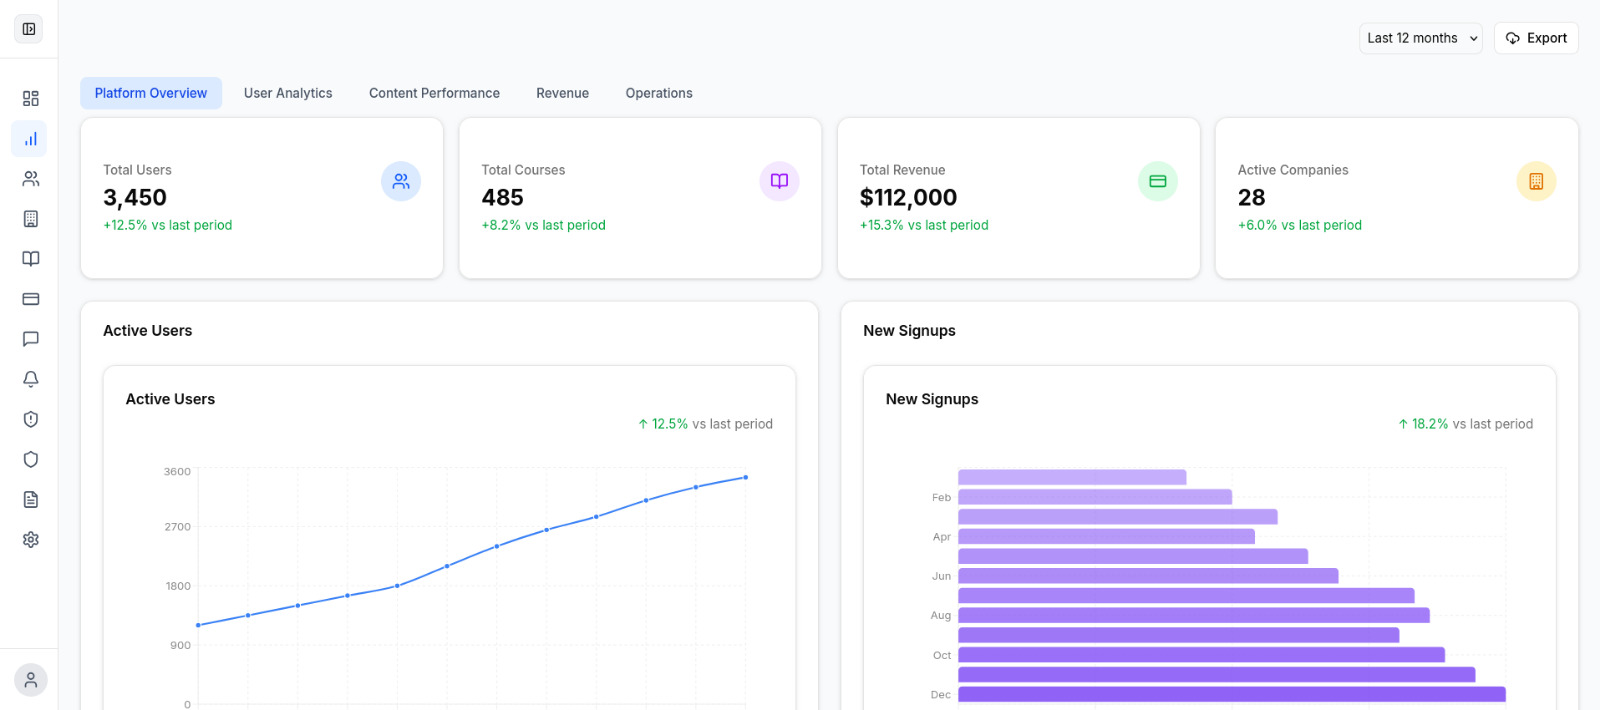
\includegraphics[width=0.85\textwidth]{anlyt.jpeg} 
  \caption{Vue d'ensemble des analyses de la plateforme pour l'administrateur.}
  \label{fig:admin_analytics}
\end{figure}

\subsubsection{Gestion des Utilisateurs}
Mise en place de l'interface de gestion des utilisateurs, permettant de visualiser la liste des utilisateurs, leurs rôles, statuts, et d'effectuer des actions de gestion. Des indicateurs clés comme le nombre total d'utilisateurs, les utilisateurs actifs et suspendus sont également affichés. (Voir Figure \ref{fig:admin_user_management}).

\begin{figure}[htbp]
  \centering
  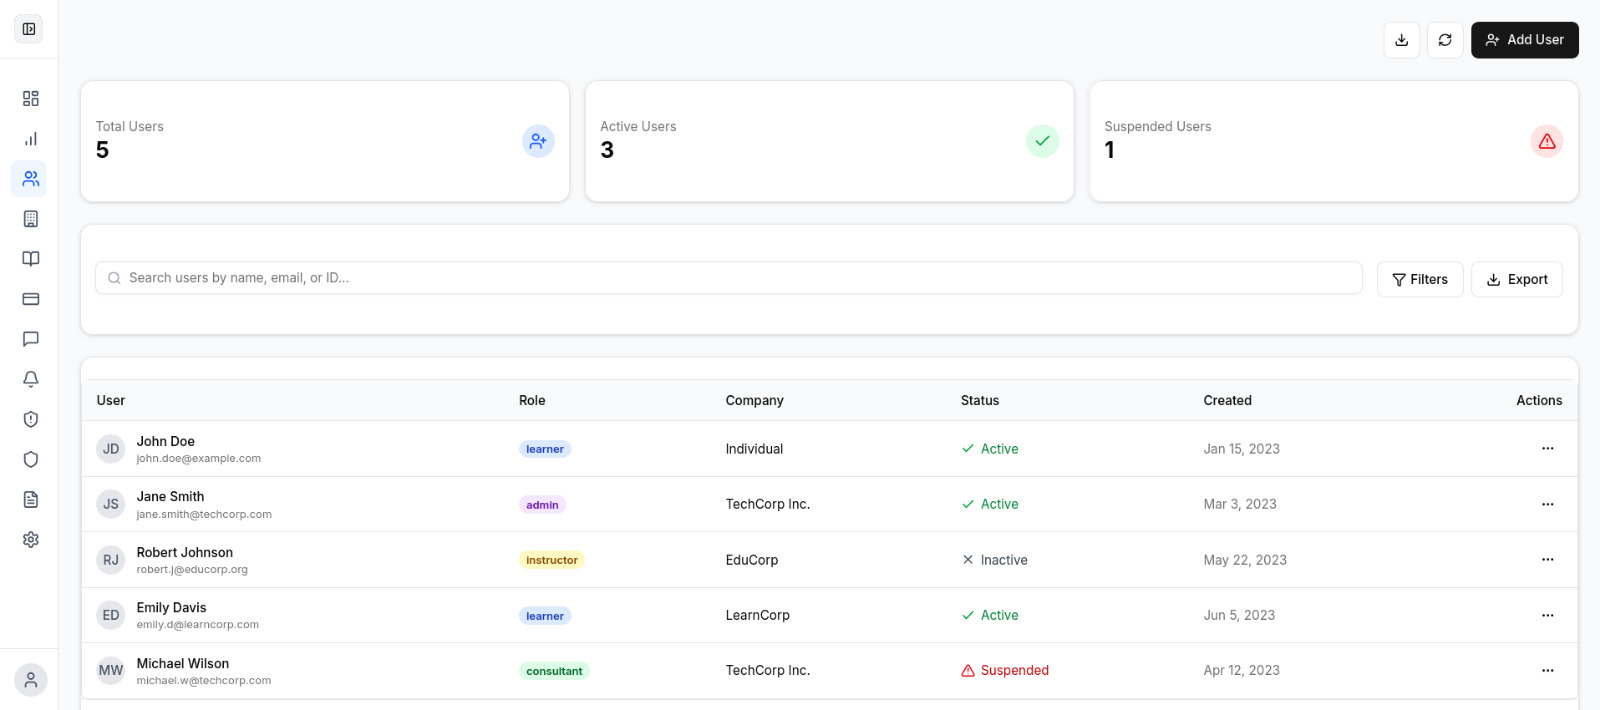
\includegraphics[width=0.85\textwidth]{usrmana.jpeg} 
  \caption{Interface de gestion des utilisateurs pour l'administrateur.}
  \label{fig:admin_user_management}
\end{figure}

\subsubsection{Gestion des Cours (Vue Administrateur)}
Finalisation de la page de gestion des cours côté administrateur, offrant une vue tabulaire des cours, avec des informations sur la catégorie, l'instructeur, le statut, le nombre d'étudiants et la note. Des options de filtrage et d'ajout de cours sont présentes. (Voir Figure \ref{fig:admin_course_management}).

\begin{figure}[htbp]
  \centering
  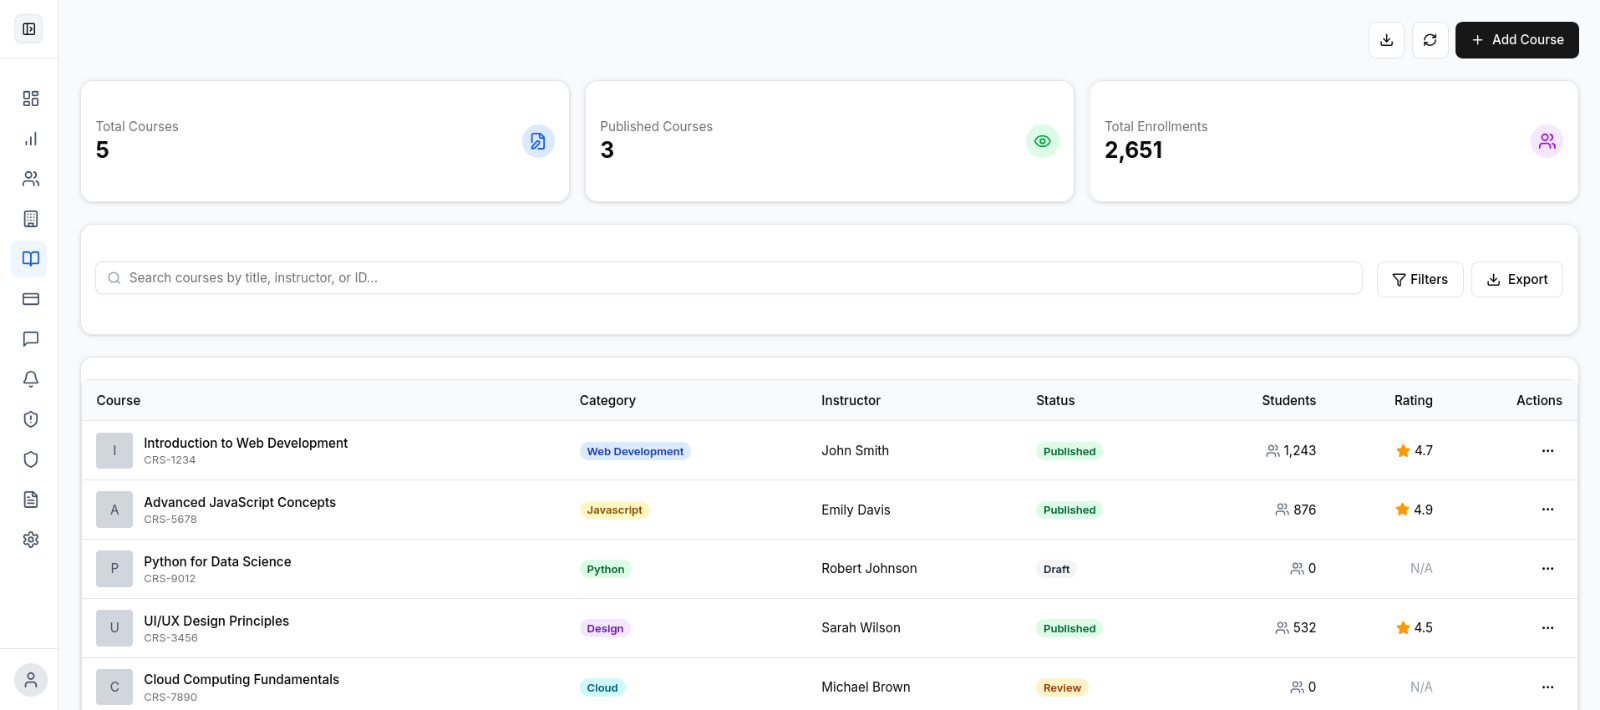
\includegraphics[width=0.85\textwidth]{coursmanagement.jpeg} 
  \caption{Interface de gestion des cours pour l'administrateur.}
  \label{fig:admin_course_management}
\end{figure}

\subsubsection{Gestion des Abonnements et de la Facturation}
Développement de l'interface pour la gestion des plans d'abonnement et le suivi de l'activité de facturation. Elle permet de visualiser les différents plans, leurs détails, et les activités récentes liées aux abonnements. (Voir Figure \ref{fig:admin_subscription_billing}).

\begin{figure}[htbp]
  \centering
  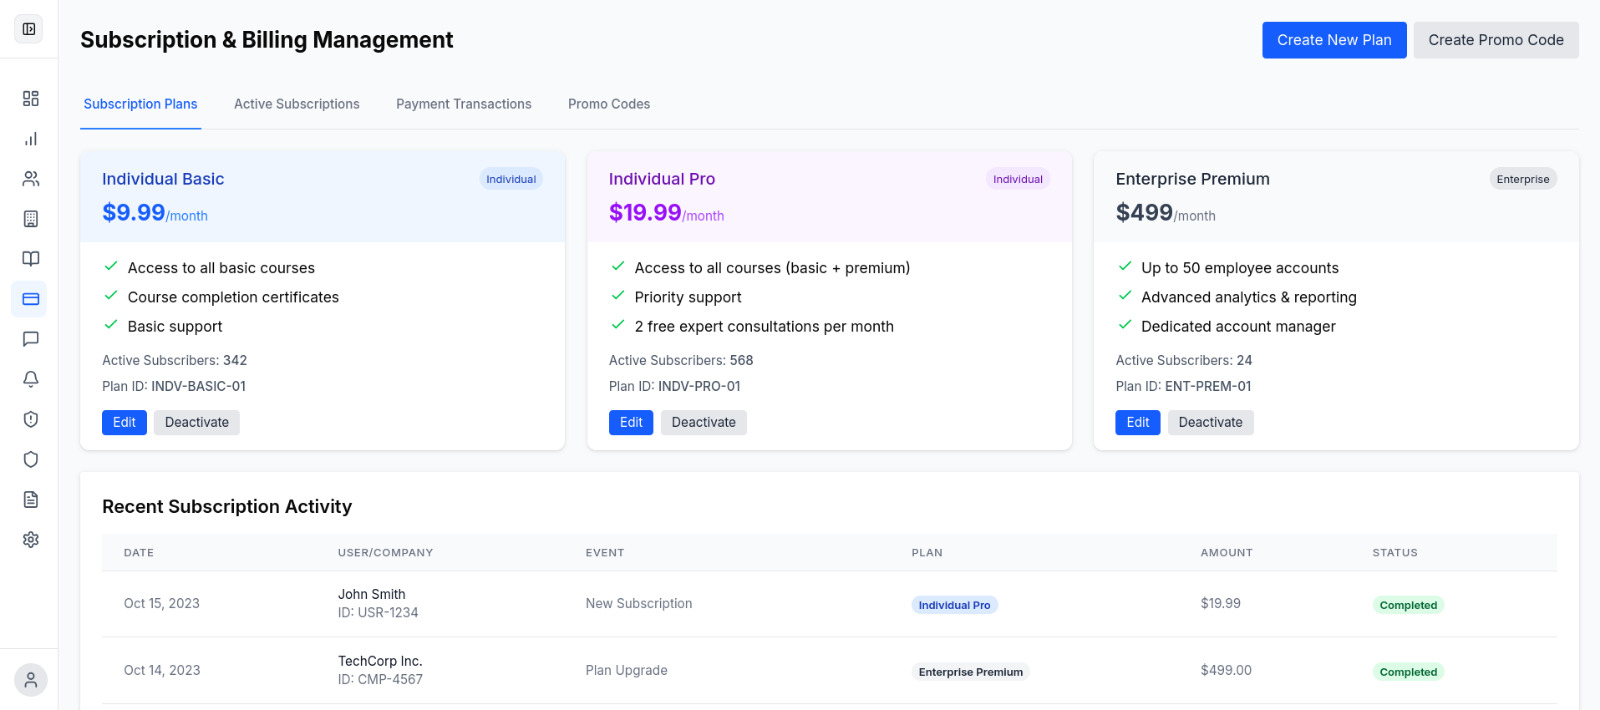
\includegraphics[width=0.85\textwidth]{sub.jpeg} 
  \caption{Interface de gestion des abonnements et de la facturation.}
  \label{fig:admin_subscription_billing}
\end{figure}

\subsubsection{Gestion des Services de Consultation}
Implémentation de la page de gestion des services de consultation, où les administrateurs peuvent définir et gérer les types de services offerts, les consultants, les sessions planifiées et visualiser les évaluations. (Voir Figure \ref{fig:admin_consultation_management}).

\begin{figure}[htbp]
  \centering
  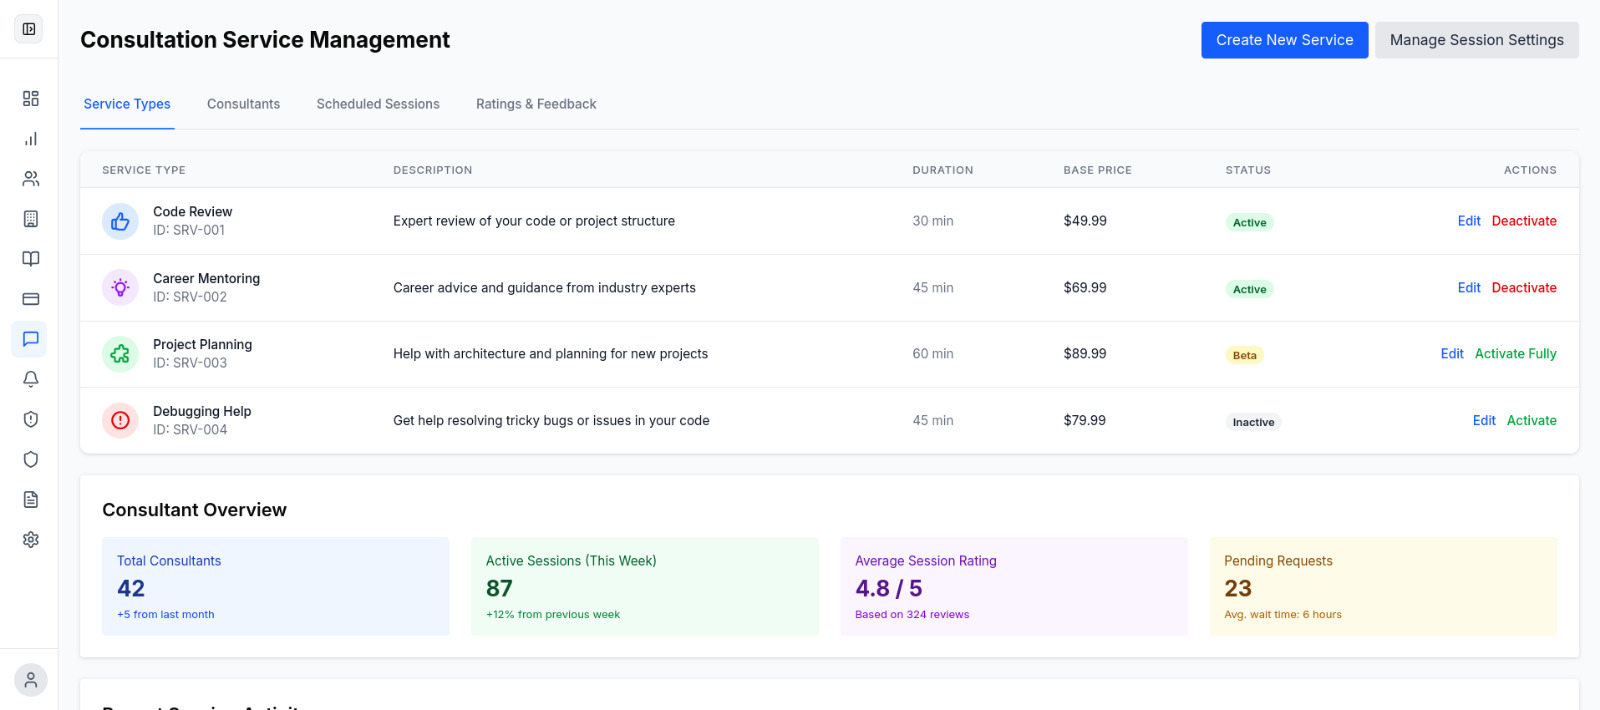
\includegraphics[width=0.85\textwidth]{consultingmana.jpeg} 
  \caption{Interface de gestion des services de consultation.}
  \label{fig:admin_consultation_management}
\end{figure}

\subsubsection{Gestion des Notifications}
Mise en place du module de gestion des notifications, permettant de créer et gérer des modèles de notification, de suivre les envois et de configurer les paramètres d'envoi. (Voir Figure \ref{fig:admin_notifications}).

\begin{figure}[htbp]
  \centering
  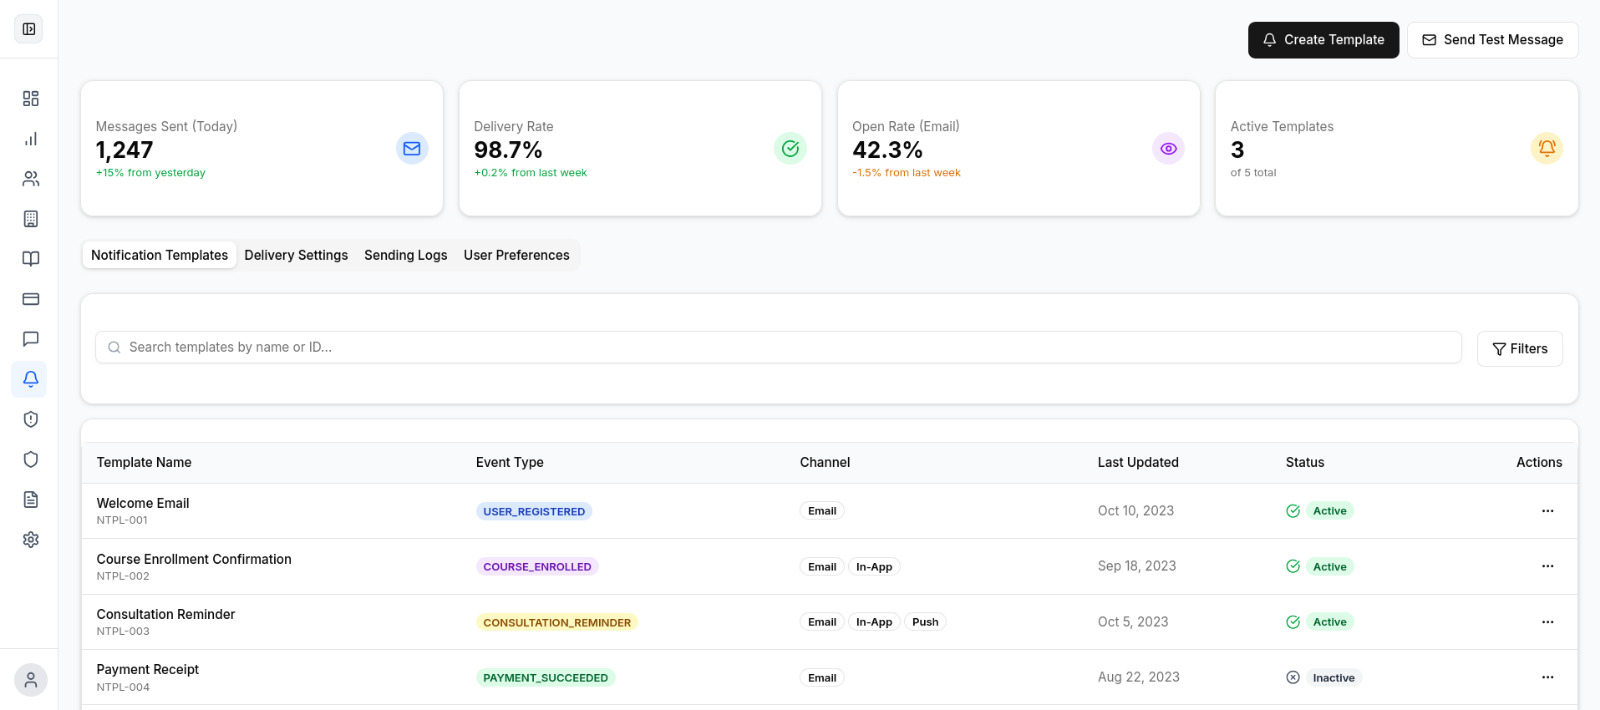
\includegraphics[width=0.85\textwidth]{notifi.jpeg} 
  \caption{Interface de gestion des modèles de notification et des envois.}
  \label{fig:admin_notifications}
\end{figure}

\subsubsection{Modération de Contenu}
Développement de l'interface de modération de contenu, affichant le contenu signalé, les révisions en attente, et les statistiques de modération, avec des options pour approuver, éditer ou supprimer le contenu. (Voir Figure \ref{fig:admin_content_moderation}).

\begin{figure}[htbp]
  \centering
  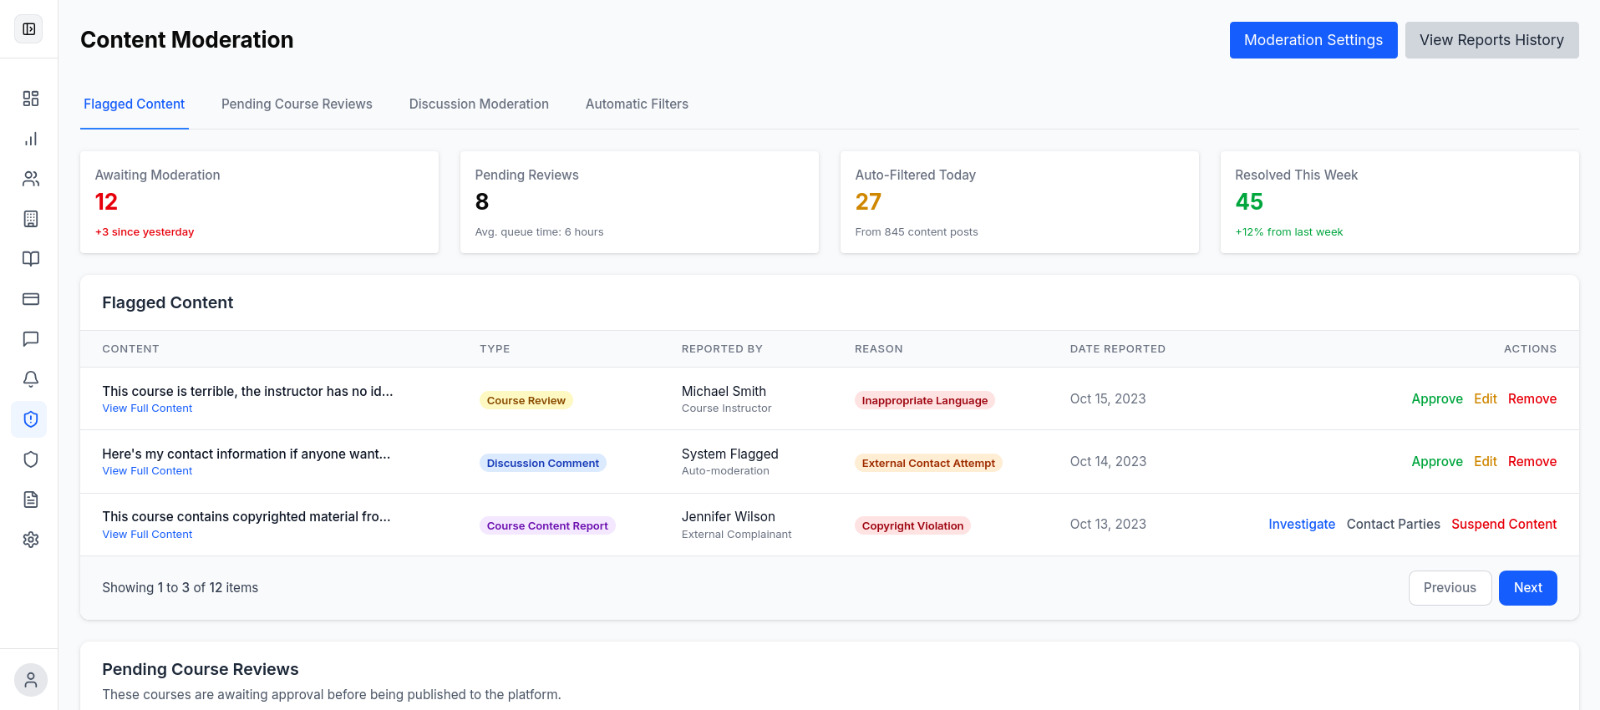
\includegraphics[width=0.85\textwidth]{contentmod.jpeg} 
  \caption{Interface de modération de contenu pour l'administrateur.}
  \label{fig:admin_content_moderation}
\end{figure}

\subsubsection{Journaux d'Audit et Suivi Système (Audit Logs)}
Création de l'interface pour la consultation des journaux d'audit, permettant de suivre les actions des utilisateurs et les événements système importants, avec des options de recherche et de filtrage. (Voir Figure \ref{fig:admin_audit_logs}).

\begin{figure}[htbp]
  \centering
  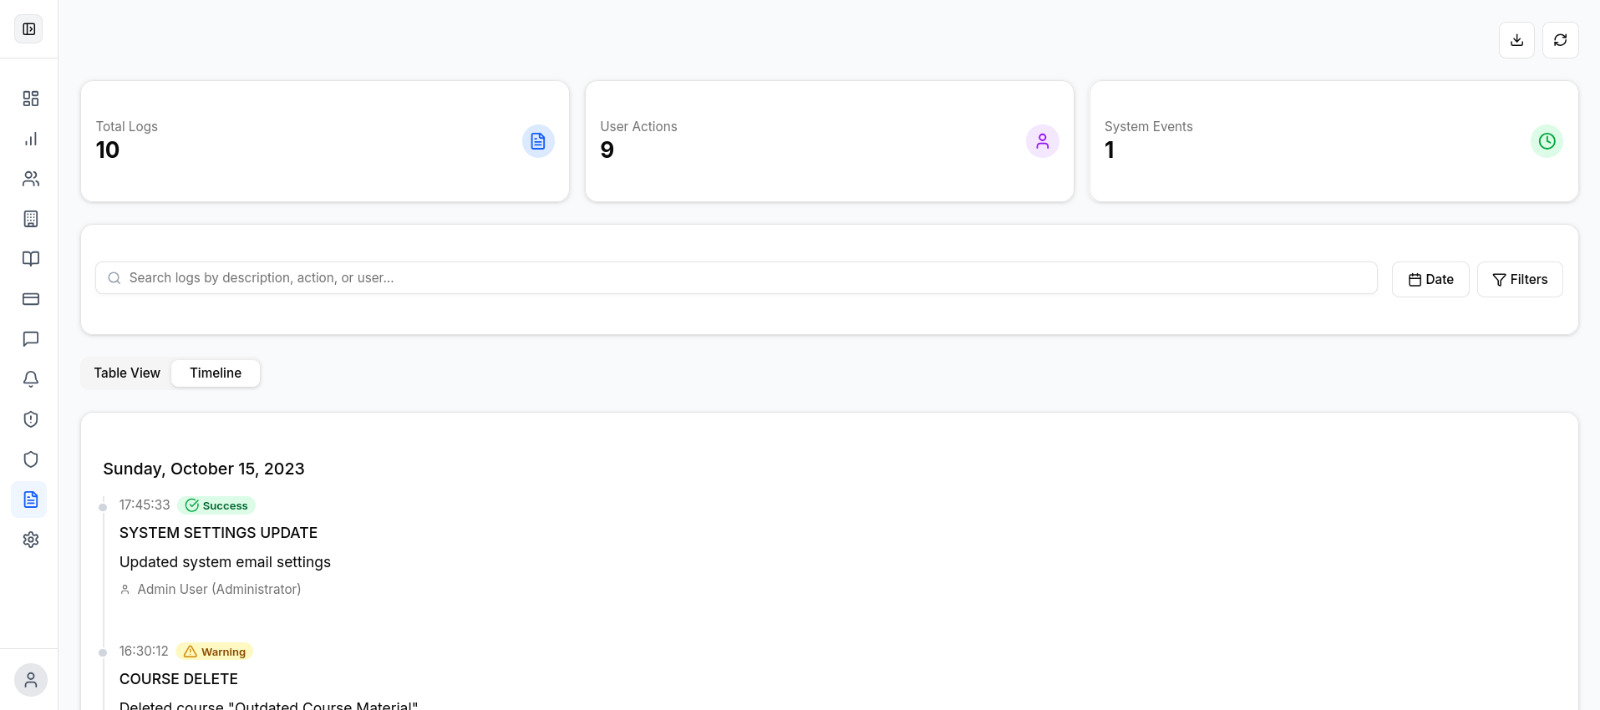
\includegraphics[width=0.85\textwidth]{audit.jpeg} 
  \caption{Interface de consultation des journaux d'audit et événements système.}
  \label{fig:admin_audit_logs}
\end{figure}

\subsubsection{Paramètres Généraux de la Plateforme}
Finalisation de la section des paramètres généraux de la plateforme, où l'administrateur peut configurer le nom de la plateforme, l'URL, la description, le fuseau horaire, le format de date, le mode maintenance, et les paramètres de contenu par défaut. (Voir Figure \ref{fig:admin_platform_settings}).

\begin{figure}[htbp]
  \centering
  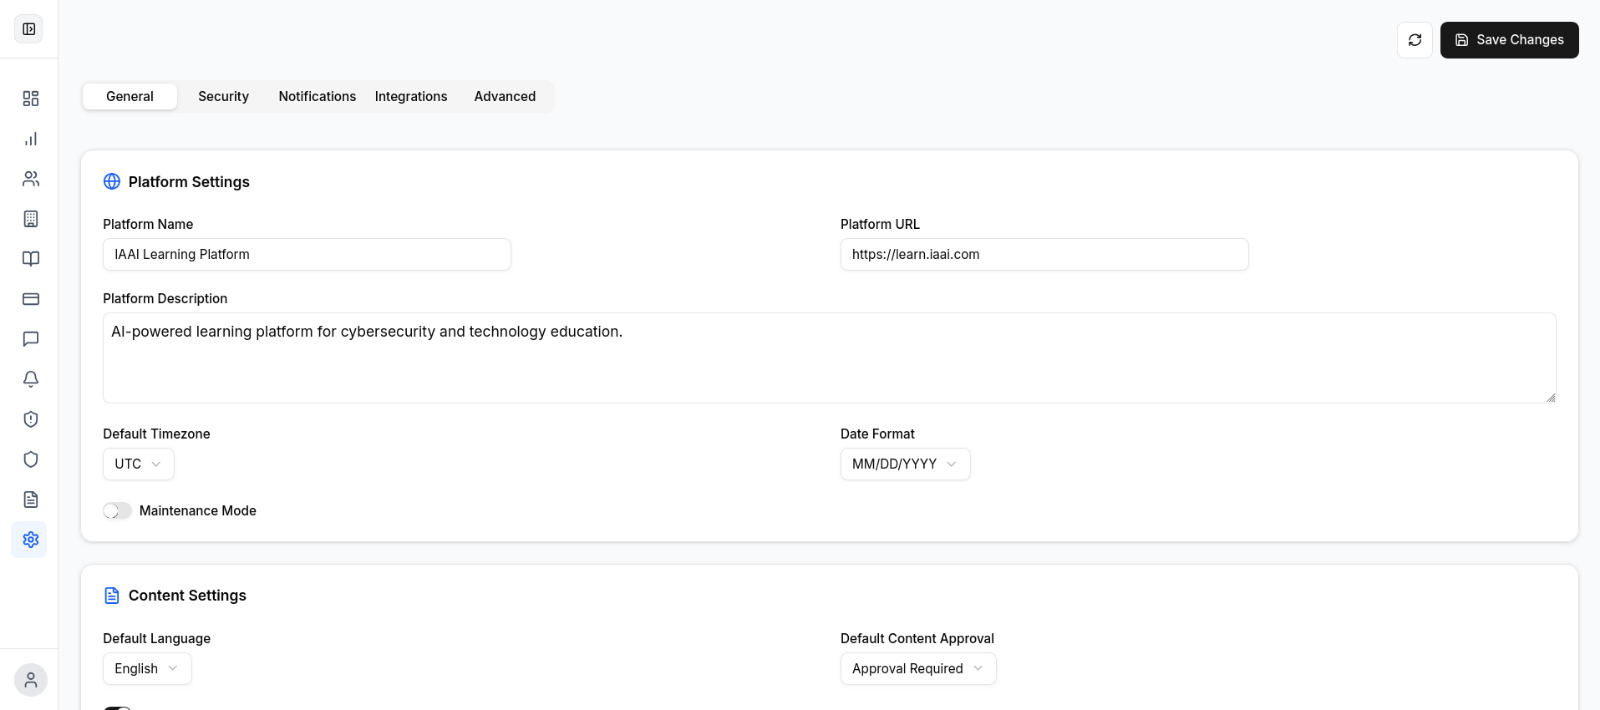
\includegraphics[width=0.85\textwidth]{settings_admin.jpeg} 
  \caption{Interface des paramètres généraux de la plateforme.}
  \label{fig:admin_platform_settings}
\end{figure}

\subsection{Philosophie de Conception pour les Interfaces Administrateur}
Comme mentionné précédemment, un choix conscient a été fait d'adopter un style d'interface utilisateur différent pour la section administrateur. L'accent a été mis sur la \textbf{clarté}, la \textbf{densité d'information pertinente} et la \textbf{fonctionnalité directe}. Pour un administrateur, l'efficacité dans le suivi et la gestion du système prime sur une esthétique très élaborée. L'objectif est de fournir des outils robustes et des indicateurs clés (insights) pour un monitoring efficace de la plateforme.

\subsection{Planification pour le Jour Suivant (Samedi 31 Mai 2025)}
Pour la journée de demain (Jour 6 de la Semaine 4), les activités prévues sont :
\begin{itemize}
  \item Poursuivre et viser la finalisation du développement des interfaces d'authentification (connexion, inscription, récupération de mot de passe, etc.).
  \item Débuter l'expérimentation et la configuration d'une passerelle API (API Gateway) en utilisant Nginx.
  \item En fonction de l'avancement sur les interfaces d'authentification et l'API Gateway, commencer la phase de conception et de planification pour le développement initial des services backend principaux de la plateforme. Cette étape préparera le terrain avant de démarrer activement le développement de ces services.
\end{itemize}

\section{Conclusion}
Cette cinquième journée conclut une semaine productive, marquée par d'importantes avancées sur les interfaces d'administration de LearnExpert. La complétion des modules d'analyse, de gestion des utilisateurs, des cours, des abonnements, des consultations, des notifications, de la modération, des logs et des paramètres généraux constitue une base solide pour la gestion de la plateforme. La philosophie de conception axée sur la fonctionnalité pour l'administration a guidé ces développements. La semaine prochaine sera consacrée aux interfaces d'authentification et à la transition vers les aspects backend, en commençant par l'infrastructure API.

\end{document}